\documentclass[letterpaper]{article}
\usepackage[letterpaper]{geometry}
\usepackage{amsmath,amsfonts,amsthm,amssymb}
\usepackage{fancyhdr}
\usepackage{enumitem}
\usepackage{extramarks}
\usepackage{chngpage}
\usepackage{graphicx,float}
\usepackage{multicol}
\usepackage{tikz,pgfplots}
\usepackage{natbib}
\usepackage{multirow,multicol}
\newcommand{\Class}{CS 1550}
\newcommand{\ClassInstructor}{Prof. Jonathan Misurda}
\newcommand{\ClassGrader}{Zhenjiang Fan}

% Homework Specific Information. Change it to your own
\newcommand{\Title}{Project 3}
\newcommand{\DueDate}{Nov. 19, 2017}
\newcommand{\StudentName}{Zac Yu}
\newcommand{\StudentLDAP}{zhy46@}

% In case you need to adjust margins:
\topmargin=-0.45in      %
\evensidemargin=0in     %
\oddsidemargin=0in      %
\textwidth=6.5in        %
\textheight=9.0in       %
\headsep=0.25in         %

% Setup the header and footer
\pagestyle{fancy}                                                       %
\lhead{\StudentName}                                                    %
\chead{\Title}                                                          %
\rhead{\firstxmark}                                                     %
\lfoot{\lastxmark}                                                      %
\cfoot{}                                                                %
\rfoot{Page\ \thepage\ of\ \protect\pageref{LastPage}}                  %
\renewcommand\headrulewidth{0.4pt}                                      %
\renewcommand\footrulewidth{0.4pt}                                      %
\renewcommand\implies\Rightarrow
\fancypagestyle{fpfancy} {
	\renewcommand{\headrulewidth}{0pt}
	%
	\fancyhf{}
	%
	\fancyfoot[L]{\lastxmark}
	%
	\fancyfoot[R]{Page\ \thepage\ of\ \protect\pageref{LastPage}}
	%
}
%%%%%%%%%%%%%%%%%%%%%%%%%%%%%%%%%%%%%%%%%%%%%%%%%%%%%%%%%%%%%
% Some tools
\newcommand{\enterProblemHeader}[1]{\nobreak\extramarks{#1}{#1 continued on next page\ldots}\nobreak%
                                    \nobreak\extramarks{#1 (continued)}{#1 continued on next page\ldots}\nobreak}%
\newcommand{\exitProblemHeader}[1]{\nobreak\extramarks{#1 (continued)}{#1 continued on next page\ldots}\nobreak%
                                   \nobreak\extramarks{#1}{}\nobreak}%

\newcommand{\homeworkProblemName}{}%
\newcounter{homeworkProblemCounter}%
\newenvironment{homeworkProblem}[1][Problem \arabic{homeworkProblemCounter}]%
  {\stepcounter{homeworkProblemCounter}%
   \renewcommand{\homeworkProblemName}{#1}%
   \section*{\homeworkProblemName}%
   \enterProblemHeader{\homeworkProblemName}}%
  {\exitProblemHeader{\homeworkProblemName}}%

\newcommand{\homeworkSectionName}{}%
\newlength{\homeworkSectionLabelLength}{}%
\newenvironment{homeworkSection}[1]%
  {% We put this space here to make sure we're not connected to the above.

   \renewcommand{\homeworkSectionName}{#1}%
   \settowidth{\homeworkSectionLabelLength}{\homeworkSectionName}%
   \addtolength{\homeworkSectionLabelLength}{0.25in}%
   \changetext{}{-\homeworkSectionLabelLength}{}{}{}%
   \subsection*{\homeworkSectionName}%
   \enterProblemHeader{\homeworkProblemName\ [\homeworkSectionName]}}%
  {\enterProblemHeader{\homeworkProblemName}%

   % We put the blank space above in order to make sure this margin
   % change doesn't happen too soon.
   \changetext{}{+\homeworkSectionLabelLength}{}{}{}}%

\newcommand{\Answer}{\ \\\textit{\textbf{Answer:}} }
\newcommand{\Proof}{\ \\\textit{\textbf{Proof:}} }
\newcommand{\Acknowledgements}[1]{\ \\{\bf Acknowledgements:} #1}
\newcommand{\Hint}[1]{\ \\{\bf Hint:} #1}
\newcommand{\Infer}{\Longrightarrow}
\newcommand{\ud}{\mathrm{d}}
\newcommand{\Reduce}{\Longleftarrow}
\newcommand{\Endproof}{\hfill $\Box$\vspace{.05in}\\}
\newcommand{\T}{\mathrm{T}}
\newcommand{\E}{\mathbb{E}}
\newcommand{\Real}{\mathbb{R}}
\newcommand*\circled[1]{\tikz[baseline=(char.base)]{\node[shape=circle,draw,inner sep=2pt] (char) {#1};}}
\renewcommand\part[1]{\textbf{(#1)}\vspace{.05in}}

%%%%%%%%%%%%%%%%%%%%%%%%%%%%%%%%%%%%%%%%%%%%%%%%%%%%%%%%%%%%%

\newcommand\hlight[1]{\tikz[overlay, remember picture,baseline=-\the\dimexpr\fontdimen22\textfont2\relax]\node[rectangle,rounded corners,draw,thick,text opacity=1] {$#1$};}
\renewcommand{\arraystretch}{1.25}
\pgfplotsset{compat=1.5}

%%%%%%%%%%%%%%%%%%%%%%%%%%%%%%%%%%%%%%%%%%%%%%%%%%%%%%%%%%%%%
% Make title
\title{\textmd{\bf \Class: \Title}\\{\large Instructed by \textit{\ClassInstructor}}\\{\vspace{-0.1in}\small Grader: \textit{\ClassGrader}}\\\normalsize\vspace{0.1in}\small{Due\ on\ \DueDate}}
%\date{} % --- if you de-comment \date{}, the date will not appear below the title
\author{\textbf{\StudentName}\ \ (LDAP: \StudentLDAP)}
%%%%%%%%%%%%%%%%%%%%%%%%%%%%%%%%%%%%%%%%%%%%%%%%%%%%%%%%%%%%%

\begin{document} % document starts here
\maketitle \thispagestyle{fpfancy}

%%%%%%%%%%%%%%%%%%%%%%%%%%%%%%%%%%%%%%%%%%%%%%%%%%%%%%%%%%%%%
% Begin edit from here

\section{VM Simulator Report}
\subsection{Abstract}
An integral part of the memory management logic of a modern Operating System is the page replacement algorithm, the algorithm to decide which page to evict out of the physical memory when it is full. Depending on the algorithm of choice, the performance (measured by the total number of page faults and number of dirty page writes) vary. In this report, we explore the performance of four different page replacement algorithms (namely ``Opt,'' ``Clock,'' ``NRU,'' and ``Random''). We do so by implementing a page table for and simulate page operations from recorded trace files of actual program execution. Finally, we speculate on the most preferable page replacement algorithm for modern OSs based on our observations.
\subsection{Implementation Overview}
\subsubsection{Page Table}
We implemented our simulated page table using a inverted page table structure (an array of simulated Page Table Entries) with cache (a hash map). We assume a 32-bit address space with each page containing $2^12=4096$ addresses (4 KB in size), and test with 8, 16, 32, and 64 frames respectively. Since the space complexity for our simulation is not a concern, we don't have to limit the size of our cache. Each inverted page table entry contains a page ID, a D (dirty) bit, and a R (referenced) bit. The page table exposes two public functions, read and write, to the user to allow simulating page read and write operations respectively. For both operation, it performs a page ID lookup in the frame (via the cache) and loads/swaps the page into the physical memory (represented by the inverted table) when necessary. It updates the dirty bits on write operations and maintains the metrics (see section~\ref{sec:metrics}) for performance measurement. Each page table is initialized with a given number of frames and an evictor (see section~\ref{sec:evictor}).
\subsubsection{Abstract Evictor}\label{sec:evictor}
When a page swap is necessary, some page replacement algorithm is responsible for choosing a page to evict out of the physical memory. We abstract the functioning unit of a page replacement algorithm by an evictor. As the name suggested, it provides a public function to suggest the page (represented by a frame ID) to evict at any given time during the simulation. In addition, it has a callback function to be called after each operation in the page table to maintain some property (e.g. to set the R bit).
\subsubsection{Optimal Evictor (\texttt{opt})}
The optimal evictor is initialized with the complete sequence of operations and precomputes the time when a page is going to be referenced next (infinity if it is not going to be used again) for each operation. During the simulation, it maintains an array of times that corresponds to when each page (load in frame) is going to be referenced next. When it is requested to suggest an evictee, it simply returns the index that has the largest value in the referenced-next array. The R bit is not used for this algorithm.
\subsubsection{Second Chance (Clock) Evictor (\texttt{clock})}
The clock evictor maintains a pointer to the frame ID to be considered as evictee next. When it is requested to suggest an evictee, it cycle through the frames, set referenced pages to be unreferenced, and return the index of the first referenced page. It also updates the R bit after each operation.
\subsubsection{Not Recently Used (NRU) Evictor (\texttt{nru})}
The NRU evictor uses a counter as a timer to clear all R bits periodically, subject to the refresh rate it is initialized with. During the simulation, after each operation, it increments the counter value, clear the R bits when appropriate, and updates the R bit of the newly referenced page to 1. When it is requested to suggest an evictee, it finds the frame that is loaded with a page with the minimum $(\texttt{RD})_2$ value.
\subsubsection{Random Evictor (\texttt{rand})}
The random evictor always returns a random (loaded) frame ID for evictee.
\subsection{Performance Analysis}
\subsubsection{Metrics}\label{sec:metrics}
We used the total number of page faults that occur during the simulation (Page Faults) and the total number of dirty frames that has to be written back to disk (Disk Writes) to measure the performance of the algorithms. Both metrics above can be implemented as variable counters in the simulated page table that increment when the corresponding actions take place.
\subsubsection{Performance Across Algorithms}\label{sec:algo}
\begin{table}
\centering
\begin{multicols}{2}
\begin{tabular}{|c|c|c|c|}
\hline
Frames              & Algo  & Page Faults & Disk Writes \\ \hline
\multirow{4}{*}{8}  & opt   & 118480      & 15030       \\ \cline{2-4} 
                    & clock & 181856      & 29401       \\ \cline{2-4} 
                    & nru   & 181092      & 19333       \\ \cline{2-4} 
                    & rand  & 216898      & 37343       \\ \hline
\multirow{4}{*}{16} & opt   & 80307       & 11314       \\ \cline{2-4} 
                    & clock & 121682      & 16376       \\ \cline{2-4} 
                    & nru   & 123710      & 13022       \\ \cline{2-4} 
                    & rand  & 150189      & 24760       \\ \hline
\multirow{4}{*}{32} & opt   & 55802       & 8266        \\ \cline{2-4} 
                    & clock & 87686       & 12293       \\ \cline{2-4} 
                    & nru   & 90990       & 9289        \\ \cline{2-4} 
                    & rand  & 106898      & 17369       \\ \hline
\multirow{4}{*}{64} & opt   & 38050       & 5725        \\ \cline{2-4} 
                    & clock & 61640       & 9346        \\ \cline{2-4} 
                    & nru   & 70481       & 6705        \\ \cline{2-4} 
                    & rand  & 74716       & 12086       \\ \hline
\end{tabular}\smallbreak
\centering{Metrics for \texttt{gcc.trace}}\columnbreak\\
\begin{tabular}{|c|c|c|c|}
\hline
Frames              & Algo  & Page Faults & Disk Writes \\ \hline
\multirow{4}{*}{8}  & opt   & 171244      & 46449       \\ \cline{2-4} 
                    & clock & 293519      & 54327       \\ \cline{2-4} 
                    & nru   & 294885      & 51943       \\ \cline{2-4} 
                    & rand  & 321308      & 54500       \\ \hline
\multirow{4}{*}{16} & opt   & 78312       & 18129       \\ \cline{2-4} 
                    & clock & 191848      & 48350       \\ \cline{2-4} 
                    & nru   & 165840      & 29760       \\ \cline{2-4} 
                    & rand  & 194614      & 40082       \\ \hline
\multirow{4}{*}{32} & opt   & 28826       & 6899        \\ \cline{2-4} 
                    & clock & 53025       & 11140       \\ \cline{2-4} 
                    & nru   & 61518       & 7778        \\ \cline{2-4} 
                    & rand  & 84050       & 18376       \\ \hline
\multirow{4}{*}{64} & opt   & 14289       & 4097        \\ \cline{2-4} 
                    & clock & 22611       & 5844        \\ \cline{2-4} 
                    & nru   & 39402       & 4707        \\ \cline{2-4} 
                    & rand  & 35244       & 8458        \\ \hline
\end{tabular}\smallbreak
\centering{Metrics for \texttt{swim.trace}}
\end{multicols}
\caption{Performance statistics across algorithms}\label{tbl:algo}
\end{table}\noindent
\begin{figure}
\centering
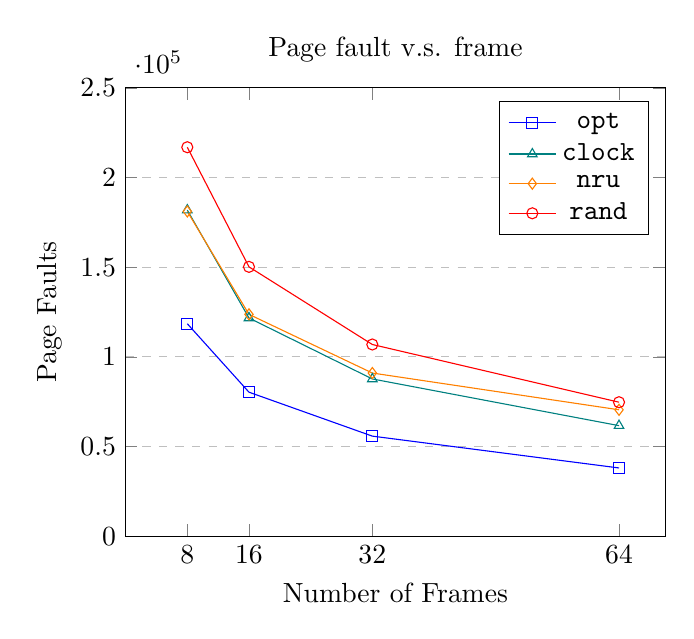
\begin{tikzpicture}
\begin{axis}[
    title={Page fault v.s. frame},
    xlabel={Number of Frames},
    ylabel={Page Faults},
    xmin=0, xmax=70,
    ymin=0, ymax=250000,
    xtick={8, 16, 32, 64},
    ytick={0,50000,100000,150000,200000,250000},
    legend pos=north east,
    ymajorgrids=true,
    grid style=dashed,
]
\addplot[color=blue, mark=square]
    coordinates {(8, 118480)(16, 80307)(32, 55802)(64, 38050)};
\addplot[color=teal, mark=triangle]
    coordinates {(8, 181856)(16, 121682)(32, 87686)(64, 61640)}; 
\addplot[color=orange, mark=diamond]
    coordinates {(8, 181092)(16, 123710)(32, 90990)(64, 70481)};
\addplot[color=red, mark=o]
    coordinates {(8, 216898)(16, 150189)(32, 106898)(64, 74716)};
\legend{\texttt{opt}, \texttt{clock}, \texttt{nru}, \texttt{rand}}
\end{axis}
\end{tikzpicture}
\quad
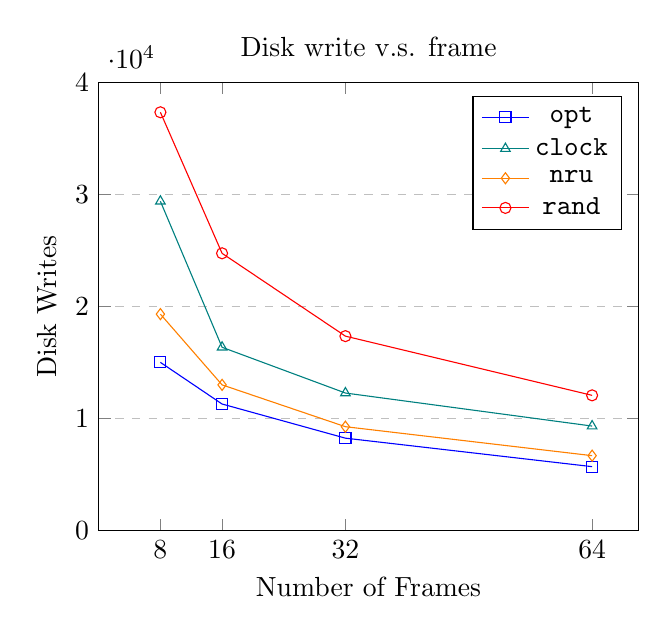
\begin{tikzpicture}
\begin{axis}[
	title={Disk write v.s. frame},
    xlabel={Number of Frames},
    ylabel={Disk Writes},
    xmin=0, xmax=70,
    ymin=0, ymax=40000,
    xtick={8, 16, 32, 64},
    ytick={0,10000,20000,30000,40000},
    legend pos=north east,
    ymajorgrids=true,
    grid style=dashed,
]
\addplot[color=blue, mark=square]
    coordinates {(8, 15030)(16, 11314)(32, 8266)(64, 5725)};
\addplot[color=teal, mark=triangle]
    coordinates {(8, 29401)(16, 16376)(32, 12293)(64, 9346)}; 
\addplot[color=orange, mark=diamond]
    coordinates {(8, 19333)(16, 13022)(32, 9289)(64, 6705)};
\addplot[color=red, mark=o]
    coordinates {(8, 37343)(16, 24760)(32, 17369)(64, 12086)};
\legend{\texttt{opt}, \texttt{clock}, \texttt{nru}, \texttt{rand}}
\end{axis}
\end{tikzpicture}
\caption{\texttt{gcc.trace} page faults and disk writes}\label{fig:gcc}
\end{figure}\noindent
Table~\ref{tbl:algo} lists the counter values, for each trace file, for each number of frames ($n$), for each algorithm (using a refresh rate of $4n$ for NRU).\\
As shown in Figure~\ref{fig:gcc}, when simulating \texttt{gcc.trace}, the optimal algorithm, as expected, yielded the fewest number of page faults and disk writes across all configurations. Conversely, the random algorithm causes more page faults and disk writes for most configurations.\\
We observed that the number of page faults resulted in by the clock algorithm and the NRU algorithm are close. However, due to clock algorithm's lack of consideration for disk writes, it generally causes significantly more disk writes when compared to the NRU algorithm.\\
It's interesting to note that the when the refresh rate is set to be strictly promotional to the number of frames, the performance of the NRU algorithm degrades over number of frames. Specifically, with 32 or 64 frames in the physical memory, the NRU algorithm's number of page faults becomes noticeably larger than that of the clock algorithm. This problem can be mitigated by finely adjusting the refresh rate accordingly to the number of frames (more in section~\ref{sec:refresh}).\\
\begin{figure}
\centering
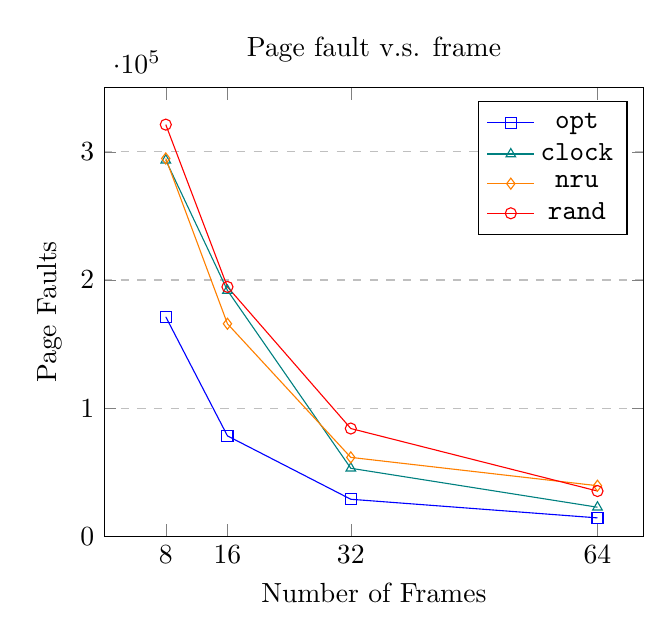
\begin{tikzpicture}
\begin{axis}[
    title={Page fault v.s. frame},
    xlabel={Number of Frames},
    ylabel={Page Faults},
    xmin=0, xmax=70,
    ymin=0, ymax=350000,
    xtick={8, 16, 32, 64},
    ytick={0,100000,200000,300000,400000},
    legend pos=north east,
    ymajorgrids=true,
    grid style=dashed,
]
\addplot[color=blue, mark=square]
    coordinates {(8, 171244)(16, 78312)(32, 28826)(64, 14289)};
\addplot[color=teal, mark=triangle]
    coordinates {(8, 293519)(16, 191848)(32, 53025)(64, 22611)}; 
\addplot[color=orange, mark=diamond]
    coordinates {(8, 294885)(16, 165840)(32, 61518)(64, 39402)};
\addplot[color=red, mark=o]
    coordinates {(8, 321308)(16, 194614)(32, 84050)(64, 35244)};
\legend{\texttt{opt}, \texttt{clock}, \texttt{nru}, \texttt{rand}}
\end{axis}
\end{tikzpicture}
\quad
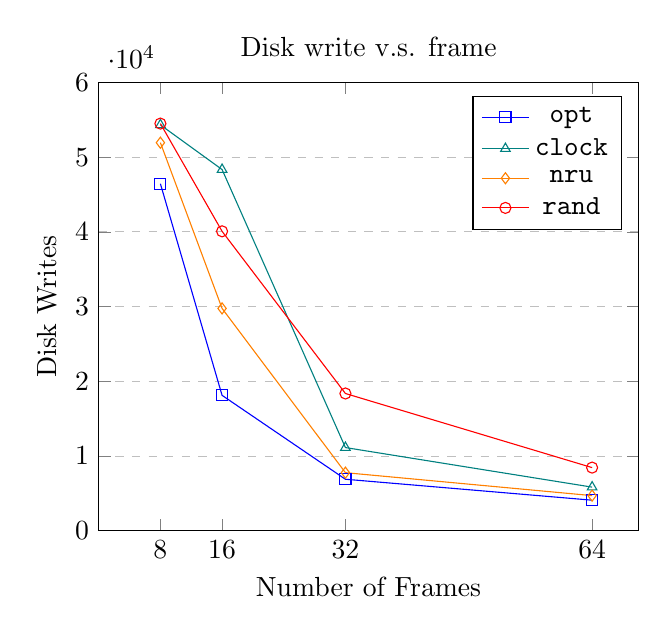
\begin{tikzpicture}
\begin{axis}[
	title={Disk write v.s. frame},
    xlabel={Number of Frames},
    ylabel={Disk Writes},
    xmin=0, xmax=70,
    ymin=0, ymax=60000,
    xtick={8, 16, 32, 64},
    ytick={0,10000,20000,30000,40000,50000,60000},
    legend pos=north east,
    ymajorgrids=true,
    grid style=dashed,
]
\addplot[color=blue, mark=square]
    coordinates {(8, 46449)(16, 18129)(32, 6899)(64, 4097)};
\addplot[color=teal, mark=triangle]
    coordinates {(8, 54327)(16, 48350)(32, 11140)(64, 5844)}; 
\addplot[color=orange, mark=diamond]
    coordinates {(8, 51943)(16, 29760)(32, 7778)(64, 4707)};
\addplot[color=red, mark=o]
    coordinates {(8, 54500)(16, 40082)(32, 18376)(64, 8458)};
\legend{\texttt{opt}, \texttt{clock}, \texttt{nru}, \texttt{rand}}
\end{axis}
\end{tikzpicture}
\caption{\texttt{swim.trace} page faults and disk writes}\label{fig:swim}
\end{figure}\noindent
In Figure~\ref{fig:swim}, we observed a similar trend for \texttt{swim.trace}. However, the performance measured by the number of page faults degrades even faster for the NRU algorithm. With 64 frames in the physical memory, the NRU algorithm performs even worse than the random algorithm (namely choosing pages to evict randomly).\\
In addition, we noticed that the number of disk writes of the clock algorithm is inconsistent. In particular, with 8 or 16 frames, the clock algorithm resulted in close to or even more disk writes than the random algorithm. Indeed, since the dirty bit is not used deciding the page to evict, there is no guarantee whatsoever.
\subsubsection{Performance Across Refresh Rate}\label{sec:refresh}
\begin{table}
\centering
\begin{multicols}{2}
\begin{tabular}{|c|c|c|c|}
\hline
Frames              & Rate & Page Faults & Disk Writes \\ \hline
\multirow{7}{*}{8}  & 16   & 174046      & 18193       \\ \cline{2-4} 
                    & 32   & 181092      & 19333       \\ \cline{2-4} 
                    & 64   & 210090      & 18586       \\ \cline{2-4} 
                    & 128  & 247677      & 17251       \\ \cline{2-4} 
                    & 256  & 283767      & 16842       \\ \cline{2-4} 
                    & 384  & 305836      & 17254       \\ \cline{2-4} 
                    & 512  & 321980      & 18678       \\ \cline{2-4} 
                    & 640  & 337768      & 20410       \\ \hline
\multirow{7}{*}{16} & 16   & 156441      & 13412       \\ \cline{2-4} 
                    & 32   & 133487      & 11998       \\ \cline{2-4} 
                    & 64   & 123710      & 9711        \\ \cline{2-4} 
                    & 128  & 144753      & 13679       \\ \cline{2-4} 
                    & 256  & 190646      & 13553       \\ \cline{2-4} 
                    & 384  & 214867      & 13231       \\ \cline{2-4} 
                    & 512  & 230018      & 12867       \\ \cline{2-4} 
                    & 640  & 244660      & 12921       \\ \hline
\multirow{7}{*}{32} & 16   & 148978      & 11273       \\ \cline{2-4} 
                    & 32   & 130396      & 10807       \\ \cline{2-4} 
                    & 64   & 104364      & 9711        \\ \cline{2-4} 
                    & 128  & 90990       & 9289        \\ \cline{2-4} 
                    & 256  & 96056       & 11106       \\ \cline{2-4} 
                    & 384  & 117962      & 11272       \\ \cline{2-4} 
                    & 512  & 137667      & 11215       \\ \cline{2-4} 
                    & 640  & 152277      & 10966       \\ \hline
\multirow{7}{*}{64} & 16   & 138512      & 9801        \\ \cline{2-4} 
                    & 32   & 123256      & 10193       \\ \cline{2-4} 
                    & 64   & 100676      & 9378        \\ \cline{2-4} 
                    & 128  & 85372       & 7951        \\ \cline{2-4} 
                    & 256  & 70481       & 6705        \\ \cline{2-4} 
                    & 384  & 64012       & 6718        \\ \cline{2-4} 
                    & 512  & 63732       & 7414        \\ \cline{2-4} 
                    & 640  & 64874       & 8024        \\ \hline
\end{tabular}\smallbreak
\centering{Metrics for \texttt{gcc.trace}}\columnbreak\\
\begin{tabular}{|c|c|c|c|}
\hline
Frames              & Rate & Page Faults & Disk Writes \\ \hline
\multirow{7}{*}{8}  & 16   & 292713      & 51575       \\ \cline{2-4} 
                    & 32   & 294885      & 51943       \\ \cline{2-4} 
                    & 64   & 307397      & 49286       \\ \cline{2-4} 
                    & 128  & 344913      & 35455       \\ \cline{2-4} 
                    & 256  & 459516      & 25246       \\ \cline{2-4} 
                    & 384  & 524616      & 21308       \\ \cline{2-4} 
                    & 512  & 556403      & 20970       \\ \cline{2-4} 
                    & 640  & 576372      & 20712       \\ \hline
\multirow{7}{*}{16} & 16   & 246505      & 28155       \\ \cline{2-4} 
                    & 32   & 180457      & 21150       \\ \cline{2-4} 
                    & 64   & 165840      & 29760       \\ \cline{2-4} 
                    & 128  & 161641      & 23756       \\ \cline{2-4} 
                    & 256  & 173624      & 17693       \\ \cline{2-4} 
                    & 384  & 189591      & 14815       \\ \cline{2-4} 
                    & 512  & 208184      & 13737       \\ \cline{2-4} 
                    & 640  & 229762      & 12693       \\ \hline
\multirow{7}{*}{32} & 16   & 241775      & 27299       \\ \cline{2-4} 
                    & 32   & 166296      & 16113       \\ \cline{2-4} 
                    & 64   & 98822       & 10759       \\ \cline{2-4} 
                    & 128  & 61518       & 7778        \\ \cline{2-4} 
                    & 256  & 54201       & 8250        \\ \cline{2-4} 
                    & 384  & 60449       & 8346        \\ \cline{2-4} 
                    & 512  & 67521       & 8143        \\ \cline{2-4} 
                    & 640  & 76486       & 7948        \\ \hline
\multirow{7}{*}{64} & 16   & 205105      & 20227       \\ \cline{2-4} 
                    & 32   & 146737      & 14302       \\ \cline{2-4} 
                    & 64   & 89813       & 9489        \\ \cline{2-4} 
                    & 128  & 56082       & 6605        \\ \cline{2-4} 
                    & 256  & 39402       & 4707        \\ \cline{2-4} 
                    & 384  & 33259       & 4364        \\ \cline{2-4} 
                    & 512  & 30364       & 4435        \\ \cline{2-4} 
                    & 640  & 29552       & 4590        \\ \hline
\end{tabular}\smallbreak
\centering{Metrics for \texttt{swim.trace}}
\end{multicols}
\caption{Performance statistics across refresh rates}\label{tbl:rate}
\end{table}\noindent
\begin{figure}
\centering
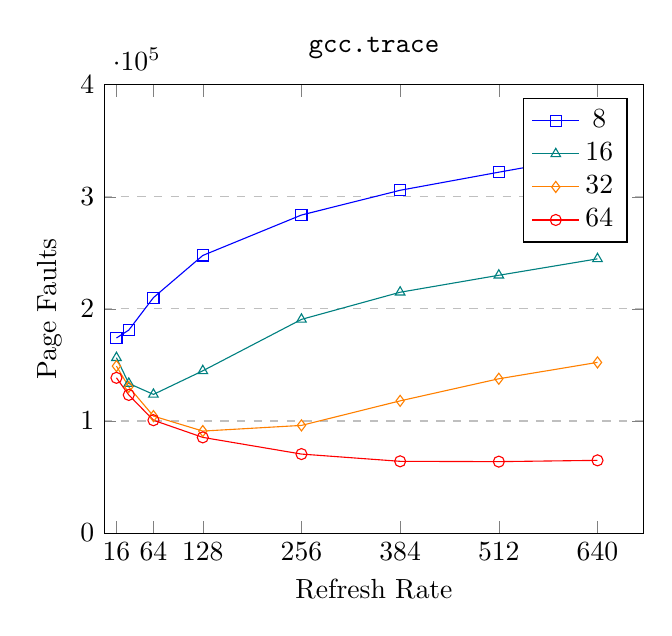
\begin{tikzpicture}
\begin{axis}[
    title={\texttt{gcc.trace}},
    xlabel={Refresh Rate},
    ylabel={Page Faults},
    xmin=0, xmax=700,
    ymin=0, ymax=400000,
    xtick={16, 64, 128, 256, 384, 512, 640},
    ytick={0,100000,200000,300000,400000},
    legend pos=north east,
    ymajorgrids=true,
    grid style=dashed,
]
\addplot[color=blue, mark=square]
    coordinates {(16, 174046)(32, 181092)(64, 210090)(128, 247677)(256, 283767)(384, 305836)(512, 321980)(640, 337768)};
\addplot[color=teal, mark=triangle]
    coordinates {(16, 156441)(32, 133487)(64, 123710)(128, 144753)(256, 190646)(384, 214867)(512, 230018)(640, 244660)}; 
\addplot[color=orange, mark=diamond]
    coordinates {(16, 148978)(32, 130396)(64, 104364)(128, 90990)(256, 96056)(384, 117962)(512, 137667)(640, 152277)}; 
\addplot[color=red, mark=o]
    coordinates {(16, 138512)(32, 123256)(64, 100676)(128, 85372)(256, 70481)(384, 64012)(512, 63732)(640, 64874)}; 
\legend{8, 16, 32, 64}
\end{axis}
\end{tikzpicture}
\quad
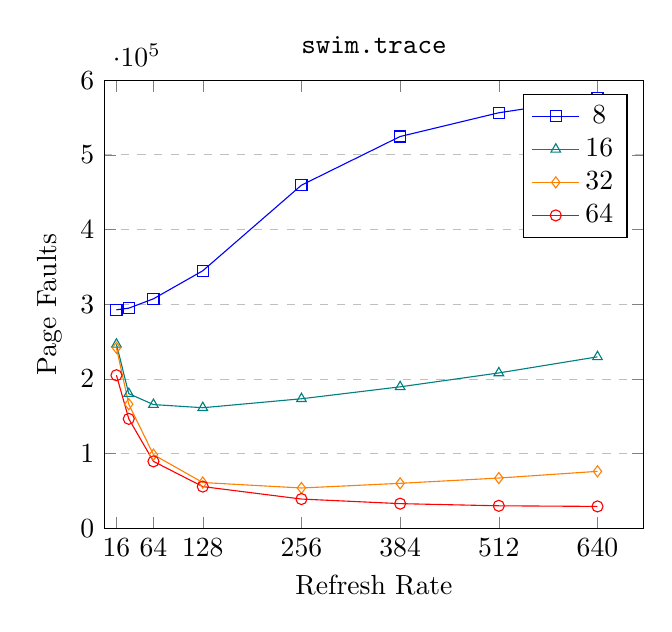
\begin{tikzpicture}
\begin{axis}[
	title={\texttt{swim.trace}},
    xlabel={Refresh Rate},
    ylabel={Page Faults},
    xmin=0, xmax=700,
    ymin=0, ymax=600000,
    xtick={16, 64, 128, 256, 384, 512, 640},
    ytick={0,100000,200000,300000,400000,500000,600000},
    legend pos=north east,
    ymajorgrids=true,
    grid style=dashed,
]
\addplot[color=blue, mark=square]
    coordinates {(16, 292713)(32, 294885)(64, 307397)(128, 344913)(256, 459516)(384, 524616)(512, 556403)(640, 576372)}; 
\addplot[color=teal, mark=triangle]
    coordinates {(16, 246505)(32, 180457)(64, 165840)(128, 161641)(256, 173624)(384, 189591)(512, 208184)(640, 229762)}; 
\addplot[color=orange, mark=diamond]
    coordinates {(16, 241775)(32, 166296)(64, 98822)(128, 61518)(256, 54201)(384, 60449)(512, 67521)(640, 76486)}; 
\addplot[color=red, mark=o]
    coordinates {(16, 205105)(32, 146737)(64, 89813)(128, 56082)(256, 39402)(384, 33259)(512, 30364)(640, 29552)}; 
\legend{8, 16, 32, 64}
\end{axis}
\end{tikzpicture}
\caption{Page fault vs. refresh rate}\label{fig:faults}
\end{figure}\noindent
Table~\ref{tbl:rate} lists the counter values, for each trace file, for each number of frames ($n$), for each refresh rate (out of 16, 32, 64, 128, 256, 384, and 512) for the NRU algorithm.\\
As shown in Figure~\ref{fig:faults}, the number of page faults with the NRU algorithm depends on the number of frames and the refresh rate. For instance, for the \texttt{gcc.trace} file, the optimal refresh rate around 16 (2x of the number of frames) for 8 frames, around 64 (4x) for 16 frames, around 128 (4x) for 32 frames, and around 512 (8x) for 64 frames. However, for the \texttt{swim.trace} file, the optimal refresh rate is around 16 (2x) for 8 frames, around 128 (8x) for 16 frames, around 256 (8x) for 32 frames, and over 640 (10x) for 64 frames.\\
We observed that the relation of the approximated optimal rate to the number of frames is not linear (faster than linear in both trace files) and varies from process to process. Based on the metrics, we propose setting the refresh rate to 4 times of the number of frames $n$ as a linear approximation for only $n<64$. This choice is also verified by our observations in Section~\ref{sec:algo} where the refresh rate is set to $4n.$
\subsection{Conclusion}
After comparing and analyzing the performance of the four (three practically implementable) page replacements algorithms, we conclude that the second chance clock algorithm is the most preferable one for modern Operating Systems. The clock algorithm consistently causes relative low number of page faults compared to the random algorithm and it does not require additional parameters such as the refresh rate for the NRU algorithm. A major downside of the NRU algorithm, other than its ineffectiveness in maintaining historical usage data, is the difficulty to determine the optimal refresh rate. As we have observed in Section~\ref{sec:refresh}, it also depends on the execution of the process itself. This leads to the consideration to have variable refresh rate per execution, which further complicates the implementation. Finally, although the NRU algorithm generally yields fewer (sometimes nearly optimal) disk writes compared to other ones, as we have acknowledged when designing the NRU algorithm (that the D bit is less significant than the R bit), the number of page faults has a greater impact on the overall performance than the number of disk writes, for which the NRU algorithm is suboptimal to the clock algorithm.
% End edit to here
%%%%%%%%%%%%%%%%%%%%%%%%%%%%%%%%%%%%%%%%%%%%%%%%%%%%%%%%%%%%%

\label{LastPage}
\end{document} % document ends here

%%%%%%%%%%%%%%%%%%%%%%%%%%%%%%%%%%%%%%%%%%%%%%%%%%%%%%%%%%%%%


